\subsection{Projektgegenstand}
\label{sec:Projektgegenstand}

Das Ziel einer möglichst ansprechenden, visuellen Darstellung des
Studienstandorts Lingen und des neuen Campus unter Verwendung moderner
Webtechnologien lässt sich auf verschiedenste Weisen realisieren. 

Um die für das Projekt geeignetste Möglichkeit der Umsetzung zu ermitteln hat
die Projektgruppe verschiedene Alternativen in Machbarkeitsstudien näher
untersucht. Hierbei unterscheiden sich die einzelnen Alternativen in
Innovativität, Attraktivität für den Anwender, und Komplexität der Umsetzung
voneinander. Konkret hat die Projektgruppe folgende Alternativen zur
Präsentation des Campus näher untersucht:

\begin{description}
\item[Fotogalerie] \hfill \\
Innerhalb einer Fotogalerie soll dem Anwender der modernisierte Studienstandort
Lingen näher gebracht werden. Zu den Fotos könnten entsprechende
Informationstexte, Beschreibungen und weiterführende Links für
Studieninteressierte hinterlegt werden.
\item[Virtueller Rundgang im Stile von Google Street View] \hfill \\
Der Anwender soll interaktiv durch Panoramafotos von den Räumlichkeiten des
Campus navigieren können. Auch bei dieser Möglichkeit der Projektrealisierung
könnten dem Nutzer weiterführende Informationen zu den abgebildeten Inhalten
präsentiert werden.
\item[Virtueller Rundgang durch ein 3D-Modell] \hfill \\
Bei dieser Möglichkeit der Umsetzug soll ein 3D-Modell des gesamten
Campusgebäude erstellt werden. Der Nutzer könnte dann virtuell duch die
modellierten Räumlichkeiten des Campus navigieren und auf diese Weise einen
Eindruck vom Studienstandort erlangen.
\end{description}

Nach der Durchführung der Machbarkeitsanalyse konnte die Projektgruppe die
Alternative der 3D-Modellierung ausschließen. Diese wurde von der Projektgruppe
als zu komplex eingestuft. Der Detaillierungsgrad, der bei der Modellierung in
der zur Verfügung stehenden Zeit erreicht werden könnte, würde nicht den
Anforderungen der Projektgruppe entsprechen. So ist es nicht möglich auf diese
Weise eine ansprechende Darstellung des Campus zu realisieren. 

Die Umsetzung als Fotogalerie wurde ebenfalls von der Projektgruppe 
ausgeschlossen. Da diese sehr schlichte Art der Präsentation nicht dem modernen
Charakter des Campus gerecht werden würde. Weiterhin vertritt die Projektgruppe
die Ansicht, dass diese Präsentationsform aufgrund von fehlender Innovation die
Zielgruppe verfehlen würde und somit keinen erheblichen Mehrwert für die
Hochschule darstellt.

Die Projektgruppe hat sich einstimmig dazu entschlossen die Projetidee durch die
Erstellung eines virtuellen Rundgangs im Stile von Google Street View zu
realisieren. Hierbei sollen die Räumlichkeiten des Campus Lingen in 360 Grad
Panoramafotos dokumentiert werden. In jedem dieser Fotos kann sich der Nutzer
frei umsehen. Auf diese Weise erhält der Nutzer einen fotorealistischen Eindruck
von den dargestellten Räumlichkeiten. Weiterhin ist es dem Nutzer möglich
selbständig durch die verschiedenen Panoramafotos zu navigieren. Hierzu werden
die einzelnen Fotos miteinander verknüpft. Mithilfe von in den Fotos
angezeigten Richtungspfeilen ist der Nutzer in der Lage sich zwischen
den verknüpften Fotos frei zu bewegen. 

Die Projektgruppe geht davon aus, dass vielen Nutzern innerhalb der Zielgruppe
diese Darstellungsform durch Google Street View bereits bekannt ist. Um von den
vorhandenen Erfahrungen der Nutzer profitieren zu können sollen bekannten
Steuerungselemente von Google Street View adaptiert werden. Diese sind in
\abbildung{GoogleStreetView} dargestellt.

\begin{figure}[htb] 
\centering
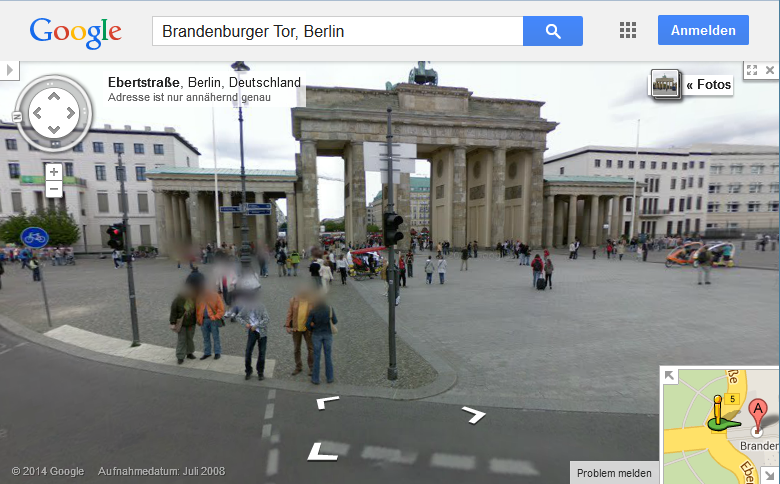
\includegraphics[width=0.7\textwidth]{GoogleStreetView.png}
\caption[Google Street View]{Google Street View\protect\footnotemark}
\label{fig:GoogleStreetView}
\end{figure}
\footnotetext{Screenshot von \url{https://maps.google.de/}}